\documentclass{beamer}

\usepackage{pri}

\graphicspath{{./}{figures/}{figures/10-links-figs/}} 

\subtitle{Web Retrieval and Link Analysis}

\begin{document}

\maketitle

% ------------------------------------------------------------

\begin{frame}
    \frametitle{Bibliography}
    
    \begin{block}{}
        \begin{itemize}
        \item \href{http://www.cs.uic.edu/~liub/WebMiningBook.html}{Bing Liu,
              Web Data Mining: Exploring Hyperlinks, Contents, and Usage Data,
              2nd edition}. Chapter 7.
        \item \href{http://www.cse.iitb.ac.in/soumen/mining-the-web/}{Christopher D. Manning, Prabhakar Raghavan and Hinrich Schütze, Introduction to Information Retrieval, Cambridge University Press}. Chapters 19 and 21.
        \item \href{http://www.mir2ed.org/}{Ricardo Baeza-Yates, Berthier
              Ribeiro-Neto, Modern Information Retrieval, 2nd edtion}. Chapter
            11.
        \end{itemize}
    \end{block}

\end{frame}

\section{Web IR vs. Traditional IR}

\begin{frame}
  \frametitle{Traditional IR}

  Traditional IR systems:
  \begin{itemize}
  \item Worth of a document regarding a query is intrinsic to the document.
  \item Documents are self-contained units
  \item Documents are descriptive and truthful
  \end{itemize}

\end{frame}

% ------------------------------------------------------------

\begin{frame}
  \frametitle{Web IR}

  The \emph{World Wide Web} is a shifting universe
  \begin{itemize}
  \item Indefinitely growing and changing
  \item Non-textual content
  \item Invisible keywords
  \item Web spam
  \item Documents are not self-complete
  \item Most web queries 2 words long
  \item \emph{Hyperlinked}
  \end{itemize}

Many features are included in a web similarity formula
  \begin{itemize}
  \item Ranking functions evaluate the reputation of pages, and different types of content within each page
  \end{itemize}
\end{frame}

% ------------------------------------------------------------

\section{The Web as a Graph}

\begin{frame}
  \frametitle{The Web as a Graph}

  \begin{itemize}
  \item The Web is an hyperlink graph
    \begin{itemize}
    \item Evolves organically,
    \item No central coordination,
    \item Yet shows global and local properties
    \item An example of a \emph{social network}
    \end{itemize}
  \end{itemize}

\end{frame}

% ------------------------------------------------------------

\begin{frame}
    \frametitle{Graph structure of the Web}
    
    \centering
    \includegraphics<+>[width=.8\linewidth]{webgraph}
    \includegraphics<+>[width=.9\linewidth]{bowtie}\\
    \only<1>{\small\href{http://www.chato.cl/papers/cdgms_2006_know_your_neighbors.pdf}{Web
        Spam detection using the web topology (Castillo et al. 2006)}}
    \only<2>{\small\href{http://www9.org/w9cdrom/160/160.html}{The Bow tie model
        (Broder et al., 2000)}}
\end{frame}

\begin{frame}
    \frametitle{A More Detailed View}    
    \centering
    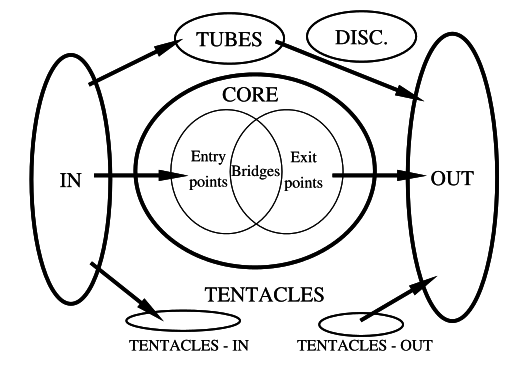
\includegraphics[width=\linewidth]{webgraph2}\\[-3ex]
    \footnotesize\href{http://doi.ieeecomputersociety.org/10.1109/SPIRE.2001.10012}{A
      study for link based web page ranking (Baeza-Yates \& Castillo, 2001)}
\end{frame}

\begin{frame}
    \frametitle{A More Recent View (cont.)}
    \begin{itemize}
    \item \emph{Bridges:} sites in CORE that can be reached directly from the IN
        component and that can reach directly the OUT component
    \item \emph{Entry points:} sites in CORE that can be reached directly from
        the IN component but are not in Bridges
    \item \emph{Exit points:} sites in CORE that reach the OUT component
        directly, but are not in Bridges
    \item \emph{Normal:} sites in CORE not belonging to the previously defined
        sub-components
    \end{itemize}
\end{frame}

% ------------------------------------------------------------

\section{Social Network Analysis}

\begin{frame}
  \frametitle{Social Network Analysis}

  \begin{itemize}
  \item Social studies based on computing properties related to \emph{connectivity and distances in graphs}
  \item Well established, long before the Web
  \item Example applications:
    \begin{itemize}
    \item Epidemiology
      \begin{itemize}
      \item Identifying a few nodes to be removed to significantly increase
        average path length between pairs of nodes
      \end{itemize}
    \item Citation analysis
      \begin{itemize}
      \item Identifying influential or central papers
      \item Identifying influential or central people
      \end{itemize}
    \end{itemize}
  \end{itemize}
  
\end{frame}

%\section{Some Examples}

\begin{frame}
    \frametitle{Finding influential researchers: H-index}
    {\small J.E. Hirsch, \textit{An index to quantify an individual's
        scientific research output}, 2005 (available
      \href{http://www.cs.ucla.edu/~palsberg/hirsch05.pdf}{\underline{here}})}
    \begin{block}{Definition}
        Index = h if h papers have at least h citations each, and the remaining
        papers have no more than h citations each.
    \end{block}
    \begin{center}
        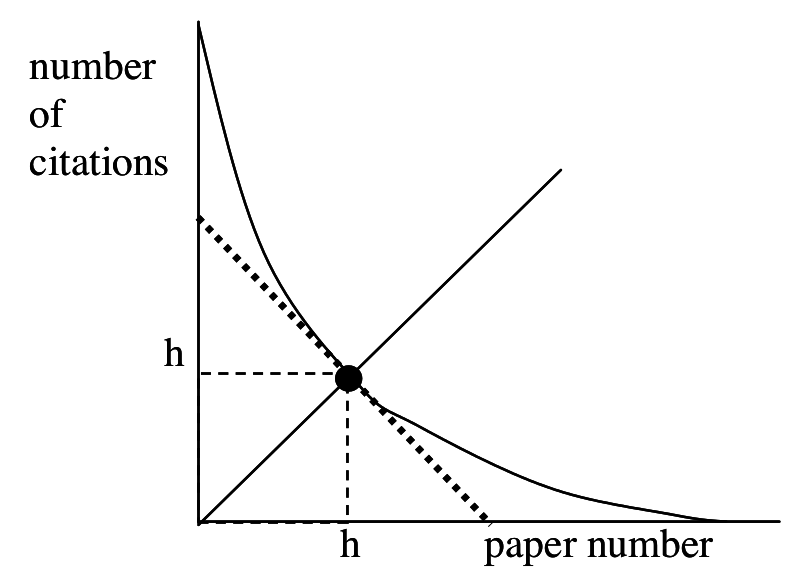
\includegraphics[width=.5\linewidth]{h-index}
    \end{center}
    \footnotesize Example: \url{http://www.cs.ucla.edu/~palsberg/h-number.html}
\end{frame}

% ------------------------------------------------------------

\begin{frame}
  \frametitle{Graph Centrality}

  \begin{itemize}
  \item Degree centrality of $v$
      \begin{itemize}
      \item Number of edges incident to $v$
      \item Directed graphs: in-degree and out-degree centrality
      \end{itemize}
  \item Betweenness centrality:
      \begin{displaymath}
          C(v) = \sum_{s \neq v \neq t}\frac{\sigma_{st}(v)}{\sigma_{st}}
      \end{displaymath}
      where $\sigma_{st} =$ \# shortest paths from $s$ to $t$ (through $v$)
  \end{itemize}

  \vfill

  Example: \url{http://onearmedman.com/research/swineflu24}

\end{frame}

\begin{frame}
  \frametitle{Topic similarity using Co-citation}

  \begin{itemize}
  \item Documents $v$ and $w$ are said to be \emph{co-cited} by $u$ if a
      document $u$ cites documents $v$ and $w$
  \item If $E$ is the document citation matrix
    \begin{itemize}
    \item $E^TE$ is the \emph{co-citation index matrix}
    \item Indicator of relatedness between every $v$ and $w$
    \end{itemize}
  \item Example use: clustering
    \begin{itemize}
    \item Using above pair-wise relatedness measure in a clustering algorithm
    \end{itemize}
  \end{itemize}

\end{frame}

% ------------------------------------------------------------

\begin{frame}
  \frametitle{Clustering with Co-citation}

  \centering
  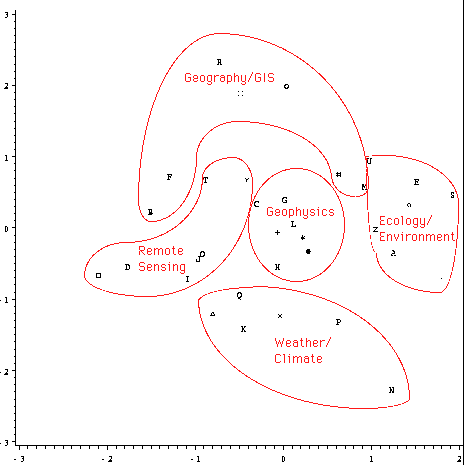
\includegraphics[width=.7\linewidth]{cocit}\\
  \tiny Social structure of Web communities
  (\href{https://sherlock.ischool.berkeley.edu/asis96/asis96.html}{source: Ray
    R. Larson}).

\end{frame}

% ------------------------------------------------------------

\section{Link Analysis and Link-based Ranking}

\begin{frame}
  \frametitle{The Web as a Graph}

  \begin{itemize}
  \item Hypermedia is a graph of documents
  \item We can apply social network theory
      \begin{itemize}
      \item Extensive research applying graph notions
      \item \emph{Centrality and prestige}
      \item \emph{Co-citation}
      \end{itemize}
  \item Application: \emph{link analysis}
  \end{itemize}

\end{frame}

\begin{frame}
    \frametitle{Link Analysis}
    Three levels of analysis:
    \begin{itemize}
    \item \emph{Macroscopic:} related to the structure of the Web at large
        \begin{itemize}
        \item E.g. the bow tie structure analysis
        \end{itemize}
    \item \emph{Mesoscopic:} related to the properties of areas or regions of
        the Web
        \begin{itemize}
        \item E.g. link-based ranking
        \end{itemize}
    \item \emph{Microscopic:} related to the statistical properties of links
        and individual nodes
        \begin{itemize}
        \item E.g. link properties
        \end{itemize}
    \end{itemize}
\end{frame}

\begin{frame}
    \frametitle{Using Link Analysis}
    Main applications:
    \begin{itemize}
    \item Prioritize crawling
    \item Identify sub-structures on the Web graph, such as \emph{communities} 
    \item \emph{Infer relevance}
    \end{itemize}
\end{frame}

\begin{frame}
  \frametitle{Link-based Ranking Strategies}
  Goal: Leverage linkage information to address the \textit{abundance problems} inherent in broad queries
  \begin{block}{Two pioneering algorithms:}
      \begin{itemize}
      \item \textbf{PageRank}: Measure of prestige for every page on web
      \item \textbf{HITS}: Identify \textit{hubs} and \textit{authorities} in a
          query result
      \end{itemize}
  \end{block}
\end{frame}

% ------------------------------------------------------------

\begin{frame}
  \frametitle{Link Model}

  \begin{itemize}
  \item Each page is a node \emph{without any textual properties}
  \item Each hyperlink is an edge connecting two nodes (possibly with an edge
      weight)
  \item Some preprocessing procedure outside the scope of the algorithm may be
      used to choose what sub-graph of the Web to analyze
  \end{itemize}

\end{frame}

% ------------------------------------------------------------

\section{PageRank}

\begin{frame}
  \frametitle{Overview}

  \begin{itemize}
  \item Pre-computes a \emph{rank-vector}
      \begin{itemize}
      \item Provides a-priori (offline) importance estimates for all pages on Web (i.e., probability distribution over pages)
      \item Independent of the search query
      \end{itemize}
  \item Prestige $\approx$ In-degree
  \item But not all votes are worth the same
  \item Prestige of a page is \emph{proportional to the sum of the prestige of
        citing pages}
  \item PageRank is \emph{part of the ranking strategy adopted by Google}
      \begin{itemize}
      \item At query time: \emph{prestige scores} used in conjunction with
          \emph{query-specific IR scores}
      \end{itemize}
  \end{itemize}

\end{frame}

% ------------------------------------------------------------

\begin{frame}
  \frametitle{PageRank Algorithm}

  The algorithm:
  \begin{itemize}
  \item E is the \textit{adjacency matrix} of the Web
    \begin{block}{}
      \begin{displaymath}
        E[u,v] = \left\{
          \begin{array}{c}
            1 \text{ iff there is a link from $u$ to $v$} \\
            0 \text{ otherwise}
          \end{array}
        \right.
      \end{displaymath}
    \end{block}
  \item The out-degree of node $u$ is given by
    \begin{block}{}
      \begin{displaymath}
        N_u = \sum_v E[u,v]
      \end{displaymath}
    \end{block}
  \item Start with an initial prestige vector $p_0[u]$
  \item Compute
    \begin{block}{}
      \begin{displaymath}
        p_{i+1}[v] = \sum_{(u,v) \in E}\frac{p_i[u]}{N_u}
      \end{displaymath}
    \end{block}
  \end{itemize}
  
\end{frame}

% ------------------------------------------------------------

\begin{frame}
    \frametitle{Main Features}
    \begin{itemize}
    \item PageRank simulates a user \emph{navigating randomly} on the Web
    \item At infinity, the probability of finding the user at any given page
        becomes stationary
    \item This process can be modeled by a \emph{Markov chain}
        \begin{itemize}
        \item stationary probability of being at each page can be computed
        \end{itemize}
    \item This probability is a property of the graph
        \begin{itemize}
        \item referred to as PageRank in the context of the Web
        \end{itemize}
    \end{itemize}
\end{frame}

\begin{frame}
  \frametitle{Convergence Conditions}

  \begin{itemize}
  \item Convergence to
    \begin{itemize}
    \item stationary distribution of the normalized adjacency matrix~$L$
    \item PageRank vector $p$ is principal eigenvector of $L$
    \end{itemize}
  \item Convergence criteria
    \begin{itemize}
    \item $L$ is \emph{irreducible}
      \begin{itemize}
      \item there is a directed path from every node to every other node
      \end{itemize}
  \item $L$ is \emph{aperiodic}
      \begin{itemize}
      \item for every node, there is no integer $k > 1$ that divides the length
          of every cycle that goes through the node
      \item the reverse---periodic---means that a node is visited always after
          a regular $nk$ number of steps ($n = 1, 2, 3, \ldots$)
          % http://www.math.chalmers.se/Stat/Grundutb/Chalmers/TMS081/oldpage/Lecture_notes/lecture3.pdf
      \end{itemize}
    \end{itemize}
  \end{itemize}

\end{frame}

% http://books.google.pt/books?id=kzXfd-ijtPoC&pg=PA104&lpg=PA104&dq=web+graph+aperiodic&source=bl&ots=LNJYRojCJf&sig=0_gWbekgYw5xrU4MjwoxX92nVns&hl=en&sa=X&ei=5JA2Uc3iE8nBOLSGgJgM&redir_esc=y#v=onepage&q=web%20graph%20aperiodic&f=false

% ------------------------------------------------------------

\begin{frame}
  \frametitle{Problems of Convergence}

  \begin{itemize}
  \item Web graph is not strongly connected
    \begin{itemize}
    \item Only a fourth of the graph is!
    \end{itemize}
  \item Web graph is not aperiodic
      \begin{itemize}
      \item There can be many periodic nodes in the Web graph
      \end{itemize}
  % \item Rank-sinks
  %   \begin{itemize}
  %   \item Pages without out-links
  %   \item Directed cyclic paths
  %   \end{itemize}
  \end{itemize}

\end{frame}

% ------------------------------------------------------------

\begin{frame}
  \frametitle{A simple fix}

  \begin{itemize}
  \item Two way choice at each node:
    \begin{itemize}
    \item With a certain probability $d$ ($0.1 < d < 0.2)$, the surfer jumps to
      a random page on the Web
    \item With probability $1-d$ the surfer decides to choose, uniformly at
      random, an out-neighbor
    \end{itemize}
    \begin{block}{}
      \begin{displaymath}
        p_{i+1}[v] = \frac{d}{N} + (1-d)\sum_{(u,v) \in E}\frac{p_i[u]}{N_u}
      \end{displaymath}
    \end{block}
  \end{itemize}

\end{frame}

% ------------------------------------------------------------

\begin{frame}
  \frametitle{PageRank architecture at Google}
  \begin{itemize}
  \item Ranking of pages more important than exact values of $p$
  \item Convergence of page ranks in 52 iterations for a crawl with 322 million
    links.
  \item Pre-compute and store the PageRank of each page.
    \begin{itemize}
    \item PageRank independent of any query or textual content.
    \end{itemize}
  \item Ranking scheme combines PageRank with textual match
    \begin{itemize}
    \item Unpublished {\it learning-to-rank} approach
    \item Many empirical parameters, human effort and regression testing.
    \end{itemize}
  \end{itemize}
\end{frame}

\begin{frame} \frametitle{Other Applications and Extensions}
\begin{itemize}
\item PageRank also used in other IR/IE applications (e.g., text summarization, keyword extraction, etc.)
\item Many extensions proposed over the years
\begin{itemize}
\item PageRank with edge weights:
\end{itemize}
      \begin{block}{}
      \begin{displaymath}
        p_{i+1}[v] = \frac{d}{N} + (1-d)\sum_{(u,v) \in E}\frac{ p_i[u] \times w(u,v) }{\sum_{(u,v') \in E} w(u,v')}
      \end{displaymath}
      \end{block}
\end{itemize}
\begin{itemize}
\item Personalized PageRank:
\end{itemize}
      \begin{displaymath}
        p_{i+1}[v] = \frac{d \times w(v)}{\sum_v' w(v)} + (1-d)\sum_{(u,v) \in E}\frac{p_i[u]}{N_u}
      \end{displaymath}
\begin{itemize}
\item Topic-sensitive PageRank, etc.
\end{itemize}
\end{itemize}
\end{frame}

% ------------------------------------------------------------

\section{HITS}

\begin{frame}
  \frametitle{HITS: Hypertext Induced Topic Selection}

  \begin{itemize}
  \item Relies on query-time processing
    \begin{itemize}
    \item To select base set $V_q$ of links for query $q$ constructed by
      \begin{itemize}
      \item selecting a sub-graph $R$ from the Web (root set) relevant to the
        query
      \item selecting any node $u$ which neighbors any $r \in R$ via an inbound
        or outbound edge (expanded set)
      \end{itemize}
    \item To deduce \emph{hubs} and \emph{authorities} that exist in a
      sub-graph of the Web
    \end{itemize}
  \item Every page $u$ has two distinct measures of merit,
    \begin{itemize}
    \item its hub score $h[u]$
    \item its authority score $a[u]$
    \end{itemize}
  \item Recursive quantitative definitions of hub and authority scores
  \end{itemize}

\end{frame}

% ------------------------------------------------------------

\begin{frame}
  \frametitle{Hubs and Authorities}

  \begin{block}{Hub}
    A page is a good hub if it contains links to many good authority pages
  \end{block}

  \begin{block}{Authority}
    A page is a good authority if it is pointed to by many good hubs
  \end{block}

  \begin{itemize}
  \item Authority pages provide good content.
  \item Hub pages provide links to the pages with good content.
  \end{itemize}

\end{frame}

% ------------------------------------------------------------

\begin{frame}
  \frametitle{The HITS Algorithm}

  ~\hspace{-.5cm}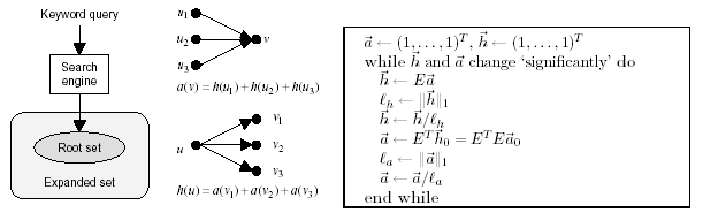
\includegraphics[width=1.2\linewidth]{hits}

\href{https://en.wikipedia.org/wiki/HITS_algorithm}  {\url{https://en.wikipedia.org/wiki/HITS_algorithm}}


\end{frame}

\begin{frame}
    \frametitle{Some Issues}
    \begin{itemize}
    \item Does not work with non-existent, repeated, or automatically generated
        links
        \begin{itemize}
        \item Solution: weigh each link based on surrounding content
        \end{itemize}
    \item \emph{Topic diffusion}
        \begin{itemize}
        \item The result set might include pages that are not directly related
            to the query
        \item One solution: associate a score with content of each page
        \item This score is then combined with the link weight
        \item Experiments show that recall and precision for first ten results
            increase significantly
        \end{itemize}
    \end{itemize}
\end{frame}

% ------------------------------------------------------------

\begin{frame}
  \frametitle{PageRank vs. HITS}

  \begin{itemize}
  \item PageRank advantage over HITS
    \begin{itemize}
    \item Query-time cost is low
      \begin{itemize}
      \item HITS computes an eigenvector for every query
      \end{itemize}
    \item Less susceptible to localized link-spam
    \end{itemize}
  \item HITS advantage over PageRank
    \begin{itemize}
    \item HITS ranking is sensitive to query
    \item HITS has notion of hubs and authorities
    \end{itemize}
  \end{itemize}

\end{frame}

\section{Web Spamming}



\begin{frame}   \frametitle{Web Spamming}

Activity of deliberately misleading a search engine by a website owner.

Deceivers try to understand how a ranking function computes, by
changing the ranking of a page without changing its user-perceived
value.

\begin{block}{SEO - Search Engine Optimization:} 
A business activity that sometimes
is legitimate, but often is not perceived as ethical.
\end{block}

\end{frame}




\begin{frame}[squeeze] \frametitle{Content Spamming}

Attempt to affect the content-based ranking features

\begin{block}{Places where to add spam terms:}

\begin{itemize}

\item Title
\item Meta-tags
\item Body
\item Anchor text
\item URL

\end{itemize}

\end{block}

\begin{block}{Techniques}
\begin{itemize}
\item repeat some important terms
 \begin{quote}the picture \emph{mining} quality of the camera
   \emph{mining} is amazing\end{quote}

\item dumping of many unrelated terms 
\begin{quote}Tom Cruise\end{quote} 

\end{itemize}
\end{block}

\end{frame}


\begin{frame}  \frametitle{Link Spamming}

\begin{itemize}
    \item out-link spamming
     \begin{itemize}
        \item easy: pick popular websites from directories
    \end{itemize}

   \item in-link spamming
   \begin{itemize}
    \item Create a honey pot
    \item Add links to web directories
    \item Post links to user-generated content sites
    \item Participate in a link exchange
    \item Create a spam farm
   \end{itemize}

\end{itemize}

\end{frame}




\begin{frame} \frametitle{Link Spamming}

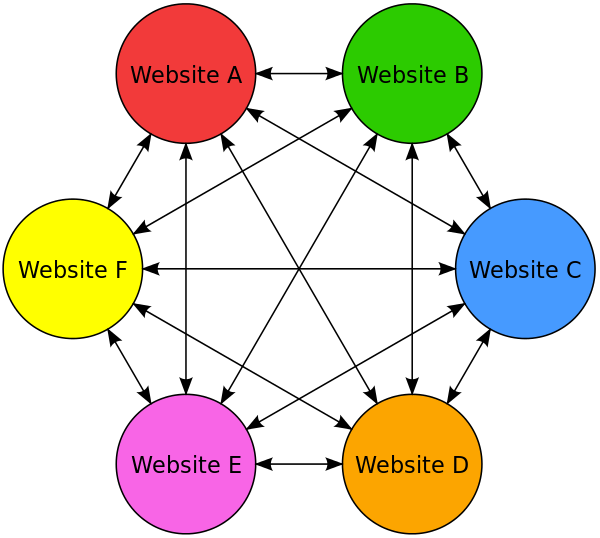
\includegraphics[width=.7\textwidth]{600px-Link_farm} 

\href{http://en.wikipedia.org/wiki/Link_farm}{\url{http://en.wikipedia.org/wiki/Link_farm}}  

 \end{frame}


\begin{frame}
  \frametitle{Hiding Techniques}

\begin{description}
\item [Content hiding:] pick background white and font color also white
\item [Cloaking:] serve one page to normal clients and another to
  search engines
\item [Redirection:] redirect browser to another page (user sees one, search engine
  will crawl both)
\end{description}

\end{frame}



\begin{frame}   \frametitle{URL Redirection}

\href{https://en.wikipedia.org/wiki/URL_redirection}  {\url{https://en.wikipedia.org/wiki/URL_redirection}}

\end{frame}



\begin{frame}   \frametitle{Combating Spam}

\begin{itemize}
\item Give higher weight to anchor text
\item PageRank - assign authority to pages based on number and importance of links
\item TrustRank - the good guys and the bad guys cluster together
\item Learn from language features common in spam (longer titles,
  longer words, ...)
\item Partition pages in blocks and compute PageRank on a block basis
  (instead of assigning a single PR value to each page), to defeat
  honeycombs and link exchanges
\item ...an on-going process... 

\end{itemize}
\end{frame}



\begin{frame} \frametitle{Click Farming}

\href{https://en.wikipedia.org/wiki/Click_farm}{\url{https://en.wikipedia.org/wiki/Click_farm}}  

\end{frame}


\begin{frame} \frametitle{The Deep Web}


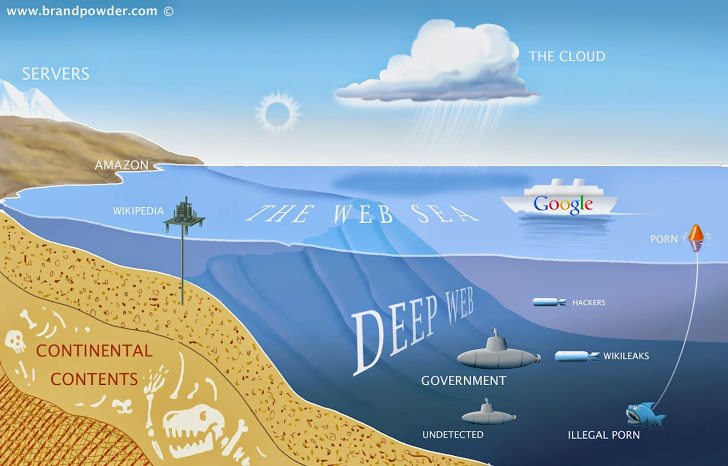
\includegraphics[width=1.0\textwidth]{deep-web.jpg} 


\small{
\href{http://thehackernews.com/2012/05/what-is-deep-web-first-trip-into-abyss.html}
        {\url{http://thehackernews.com/2012/05/what-is-deep-web-first-trip-into-abyss.html}}  
}

\end{frame}

% ------------------------------------------------------------
% ------------------------------------------------------------

\finalframe{Questions?}

\end{document}
